%input macros (i.e. write your own macros file called MacroFile1.tex)
%\include{Macros/MacroFile1}
\documentclass[oneside,12pt]{IIScthesisPSnPDF}
% \pagestyle{bfheadings}
%\usepackage{psfig}
% \usepackage{graphicx}
\usepackage{amssymb}
\usepackage{amsmath}
\usepackage{latexsym}
\usepackage{multicol}
\usepackage{booktabs}
\usepackage{multirow}
\usepackage{fancyhdr}
\usepackage[numbers]{natbib}
\usepackage{cleveref}
\usepackage{wrapfig}
\usepackage{algorithm}
\usepackage{algorithmic}
\usepackage{enumerate}
\usepackage{cancel}
\usepackage{mathrsfs}
% \usepackage{sfgame}
%\usepackage{color}
\usepackage[compact]{titlesec}
\usepackage{mdwlist}
\usepackage{tikz}
\usepackage{varwidth}
\usepackage[vertfit]{breakurl}
\usepackage{datetime}
\usepackage{pdfpages}
% \usepackage{biblatex}
\usetikzlibrary{shapes,arrows, trees}

\usepackage{epsfig,subfig,graphicx}
\usepackage{xcolor,colortbl}

%This command reserves a whole page for a figure
%Its only argument is the caption
\newcommand{\fullpagefigspace}[2]{
\begin{figure}
\vspace{5.0in}
\caption{#1}
\label{#2}
\end{figure}
}
%            
%
\newcommand{\abs}[1]{$|{#1}|$}
\newcommand{\absq}[1]{$|{#1} |^{2}$}
\newcommand{\tabs}[1]{|{#1}|}
\newcommand{\tabsq}[1]{|{#1}|^2}
\newcommand{\half}{$\frac{1}{2}$}
\newcommand{\nth}{^{\mathrm{th}}}
\newcommand{\prob}[1]{\mathsf{Pr}\left(#1\right)}
\newcommand{\EXP}[1]{\mathsf{E}\!\left(#1\right)}
\newcommand{\D}{\displaystyle}
%%%%%%%%%%%%%%%%%%%%%%%%%%%%%%%%%%%%%%%%%%%%%%%%%%%%%%%%%%%%%%%%%%%%%%%%
%THE FOLLOWING IS FOR MAKING THE CAPTIONS IN SANS SERIF AND PUT A FIGRULE
%%%%%%%%%%%%%%%%%%%%%%%%%%%%%%%%%%%%%%%%%%%%%%%%%%%%%%%%%%%%%%%%%%%%%%%%
%\newcommand{\captionfonts}{\sf}

%\makeatletter  % Allow the use of @ in command names
%\long\def\@makecaption#1#2{%
%  \vskip\abovecaptionskip
%  \sbox\@tempboxa{{\captionfonts #1: #2}}%
%  \ifdim \wd\@tempboxa >\hsize
%    {\captionfonts #1: #2\par}
%  \else
%    \hbox to\hsize{\hfil\box\@tempboxa\hfil}%
%  \fi
%  \vskip\belowcaptionskip 
%  %\figrule{138mm}
%  }
%\makeatother   % Cancel the effect of \makeatletter
%%%%%%%%%%%%%%%%%%%%%%%%%%%%%%%%%%%%%%%%%%%%%%%%%%%%%%%%%%%%%%%%%%%%%%%%
%END OF MAKING THE CAPTIONS SANS SERIF
%%%%%%%%%%%%%%%%%%%%%%%%%%%%%%%%%%%%%%%%%%%%%%%%%%%%%%%%%%%%%%%%%%%%%%%%



\newcommand{\erf}[1]{
{\mbox{\mathsf{erf}}}\left( {#1} \right)
}

\newcommand{\erfc}[1]{
{\mbox{\mathsf{erfc}}}\left( {#1} \right)
}

\newcommand{\binomial}[2]{
\left(\! {{#1}\atop{#2}}\!\right)}

%Numbered environments
\newtheorem{remarks}{Remarks}[chapter] %\label{rmk:}
\newtheorem{example}{Example}[chapter] %\label{exp:}
\newtheorem{theorem}{Theorem}[chapter]
\newtheorem{lemma}{Lemma}[chapter]
\newtheorem{corollary}{Corollary}[chapter]
\newtheorem{discussion}{Discussion}[chapter] %\label{dis:}
\newtheorem{definition}{Definition}[chapter]
\newtheorem{proposition}{Proposition}[chapter]
\newtheorem{mechanism}{Mechanism}[chapter]
\newtheorem{question}{Question}[chapter]
\newtheorem{observation}{Observation}[chapter]
\newtheorem{fact}{Fact}[chapter]
\newcommand{\remove}[1]{}

\DeclareMathOperator*{\argmin}{\arg\!\min}
\DeclareMathOperator*{\argmax}{\arg\!\max}

\newenvironment{proof}{\noindent{\bf Proof:} \hspace*{1mm}}{\hfill $\Box$ }
\newcommand{\notes}[1]{}
\newcommand{\argument}[1]{\noindent{\bf Argument: }#1 \hfill $\Box$}
\newcommand{\VAR}[1]{\mathsf{Var}\!\left(#1\right)} 
\newcommand{\bmath}[1]{\mbox{\boldmath$#1$}}
\newcommand{\first}[1]{$1^{\mathrm{st}}$}
\newcommand{\second}[1]{$2^{\mathrm{nd}}$}
\newcommand{\qed}{\hfill \rule{2.5mm}{2.5mm}}
\def\QED{\mbox{\rule[0pt]{1ex}{1ex}}}
\def\Q{\hspace*{\fill}~\QED\par\endtrivlist\unskip}
\newcommand{\mech}{{\sc VCPM}}
\newcommand{\mechA}{{\sc MATRIX}}
\newcommand{\squishlisttwo}{
\begin{list}{$\blacktriangleright$}
{ \setlength{\itemsep}{0.5pt}
\setlength{\parsep}{0pt}
\setlength{\topsep}{0pt}
\setlength{\partopsep}{0.5pt}
\setlength{\leftmargin}{1em}
\setlength{\labelwidth}{1em}
\setlength{\labelsep}{0.5em} } }

\newcommand{\squishend}{
\end{list} }
\allowdisplaybreaks[1]


% \newcommand{\nobibentry}[1]{{\let\nocite\ignore\bibentry{#1}}}
\newdateformat{monthyeardate}{ \monthname[\THEMONTH], \THEYEAR}
\newcommand{\sn}[1]  {\noindent \textcolor{blue}{{\bf SN: }{``{\em #1}''}}}
\newcommand{\blankpage}{
\newpage
\thispagestyle{empty}
\mbox{}
\newpage
}

\newcommand{\blankpagewithnumber}{
\newpage
% \thispagestyle{empty}
\mbox{}
\newpage
}

\crefname{observation}{observation}{observations}
\crefname{algorithm}{algorithm}{algorithms}
\crefname{align}{equation}{equations}
\crefname{eqnarray}{equation}{equations}

% turn of those nasty overfull and underfull hboxes
\hbadness=10000
\hfuzz=50pt

% Put all the style files you want in the directory StyleFiles and usepackage like this:
% \usepackage{StyleFiles/watermark}

% Comment out the next line to get single spacing
\onehalfspacing

\newcommand{\model}{DRAM\_HARD}
\newcommand{\modelExplicit}{DRAM\_SOFT}
\newcommand{\modelPcmRam}{PCM\_RAM}
\newcommand{\hashsize}{H}
\newcommand{\aggsize}{A}
\newcommand{\hjcount}{N_j}
\newcommand{\gbcount}{N_g}
\newcommand{\hjlen}{L_j}
\newcommand{\gblen}{L_g}
\newcommand{\FlashsortWrites} {W_{sort\_uniform}}
\newcommand{\MPFlashsortWrites} {W_{sort\_non\_uniform}}

\def\baselinestretch{1.5} 
\definecolor{c1}{RGB}{239,247,245}
\definecolor{c2}{RGB}{188,189,220}
\definecolor{c3}{RGB}{117,107,177}
\newcolumntype{x}{>{\columncolor{c1}}c}
\newcolumntype{y}{>{\columncolor{c2}}c}
\newcolumntype{z}{>{\columncolor{c3}}c}

\begin{document}

\title{On Improving Write Performance in PCM Databases} 

\submitdate{\monthyeardate\today} 
\me
%\phd
%\mscengg
%\degree{Master of Engineering} 
\dept{Supercomputer Education & Research Centre}
\faculty{Faculty of Engineering}
\author{Your Name}

% Using the watermark package which is in StyleFiles/
% and to remove DRAFT COPY ONLY appearing on the top of all pages comment out below line
%\watermark{DRAFT COPY ONLY}


\maketitle


\begin{center}
\LARGE{\underline{\textbf{Declaration of Originality}}}
\end{center}
\noindent I, \textbf{Name}, with SR No. \textbf{SR-No} hereby declare that
the material presented in the thesis titled

\begin{center}
\textbf{Thesis Title}
\end{center}

\noindent represents original work carried out by me in the \textbf{Deparment
of Computer Science and Automation} at \textbf{Indian Institute of
Science} during the years \textbf{Years}.

\noindent With my signature, I certify that:
\begin{itemize}
	\item I have not manipulated any of the data or results.
	\item I have not committed any plagiarism of intellectual
	property.
	I have clearly indicated and referenced the contributions of
	others.
	\item I have explicitly acknowledged all collaborative research
	and discusions.
	\item I have understood that any false claim will result in severe
	disciplinary action.
	\item I have understood that the work may be screened for any form
	of academic misconduct.
\end{itemize}

\vspace{20mm}

\noindent {\footnotesize{Date:	\hfill	Student Signature}} \qquad

\vspace{20mm}

\noindent In my capacity as supervisor of the above-mentioned work, I certify
that the above statements are true to the best of my knowledge, and 
I have carried out due diligence to ensure the originality of the
report.

\vspace{20mm}

\noindent  {\footnotesize{Advisor Name: \hfill Advisor Signature}} \qquad



\blankpage

\vspace*{\fill}
\begin{center}
\large\bf \textcopyright \ Your Name\\
\large\bf \monthyeardate\today\\
\large\bf All rights reserved
\end{center}
\vspace*{\fill}
\thispagestyle{empty}

\blankpage

\vspace*{\fill}
\begin{center}
DEDICATED TO \\[2em]
\Large\it The Student Community\\[2em]
\Large\it who can use and reuse this template to glory
\end{center}
\vspace*{\fill}
\thispagestyle{empty}

%\blankpage
%\includepdf[pages={1}]{declaration.pdf}

%\vspace*{\fill}
%\begin{tabular}{p{0.4\columnwidth}p{0.5\columnwidth}}
% {\em Signature of the Author}: & \dotfill \\
% & Your Name \\
% & Dept.\ of Computer Science and Automation \\ 
% & Indian Institute of Science, Bangalore \vspace{1in}\\
% {\em Signature of the Thesis Supervisor}: & \dotfill \\
% & Your Advisor's Name \\
% & Professor \\
% & Dept.\ of Computer Science and Automation \\ 
% & Indian Institute of Science, Bangalore
%\end{tabular}
%\vspace*{\fill}
%\thispagestyle{empty}

%\blankpage

%set the number of sectioning levels that get number and appear in the contents
\setcounter{secnumdepth}{3}
\setcounter{tocdepth}{3}

\frontmatter % book mode only
\pagenumbering{roman}


% \include{Dedication/dedication}
\prefacesection{Acknowledgements}
% \input{acknowledgments}

\prefacesection{Abstract}
Phase Change Memory (PCM) is a new \emph{non-volatile} memory technology
that is comparable to traditional DRAM with regard to read latency,
and markedly superior with regard to storage density and idle
power consumption. Due to these desirable characteristics, PCM is
expected to play a significant role in the next generation of computing
systems. However, it also has limitations in the form of expensive writes
and limited write endurance. Accordingly, recent research has investigated
how database engines may be redesigned to suit DBMS deployments on the
new technology.

In this paper, we address the pragmatic goal of minimally altering current
implementations of database operators to make them PCM-conscious,
the objective being to facilitate an easy transition to the new
technology. Specifically, we target the implementations of the
``workhorse'' database operators: \emph{sort}, \emph{hash join} and
\emph{group-by}, and rework them to substantively improve the write
performance without compromising on execution times. Concurrently, we
provide simple but effective \emph{estimators} of the writes incurred
by the new techniques, and these estimators are leveraged for 
integration with the query optimizer.

Our new techniques are evaluated on TPC-H benchmark queries with
regard to the following metrics: number of writes, response times and wear distribution. The experimental results indicate that the PCM-conscious
operators collectively reduce the number of writes by a factor of 2 to
3, while concurrently improving the query response times by about 20\% to
30\%.  When combined with the appropriate plan choices, the improvements
are even higher.  In essence, our algorithms provide both short-term and
long-term benefits.  These outcomes augur well for database engines that
wish to leverage the impending transition to PCM-based computing.


\prefacesection{Publications based on this Thesis}
% \input{publications}
\tableofcontents
%\blankpagewithnumber
\listoffigures
\listoftables
%\blankpagewithnumber
% \printnomenclature  %% Print the nomenclature
% \addcontentsline{toc}{chapter}{Nomenclature}

\mainmatter % book mode only
\setcounter{page}{1}
\chapter{Introduction}
\section{Introduction}
\label{sec:intro}
%
Phase Change Memory (PCM) is a recently developed non-volatile memory
technology, constructed from chalcogenide glass material, that stores
data by switching between amorphous (\emph{binary 0}) and crystalline 
(\emph{binary 1}) states. Broadly speaking, it is expected to provide an attractive
combination of the best features of conventional disks (persistence,
capacity) and of DRAM (access speed). For instance, it is
about 2 to 4 times denser than DRAM, while providing a DRAM-comparable
read latency.  On the other hand, it consumes much less energy
than magnetic hard disks while providing substantively smaller write latency. Due to this suite of  desirable features, PCM technology is
expected to play a prominent role in the next generation of computing
systems, either augmenting or replacing current components in the memory
hierarchy~\cite{qureshi,zhou,lee}.

A limitation of PCM, however, is that there is a significant difference
between the read and write behaviors in terms of energy, latency and
bandwidth. A PCM write, for example, consumes 6 times more energy than
a read. Further, PCM has limited write endurance since a memory cell
becomes unusable after the number of writes to the cell exceeds a threshold
determined by the underlying glass material. Consequently, several database
researchers have, in recent times, focused their attention on devising
new implementations of the core database operators that are adapted to
the idiosyncrasies of the PCM environment (e.g.~\cite{chen,viglas}). 

\subsection*{Architectural Model}
The prior database work has primarily focused on computing
architectures wherein either (a) PCM completely replaces the
DRAM memory~\cite{chen}; or (b) PCM and DRAM co-exist side-by-side
and are independently controlled by the software~\cite{viglas}. We
hereafter refer to these options as {\bf \modelPcmRam{}} and
{\bf \modelExplicit{}}, respectively.

However, a third option that is gaining favor in the architecture
community, and also mooted in \cite{chen} from the database
perspective, is where the PCM is augmented with a small hardware-managed
DRAM buffer~\cite{qureshi}. In this model, which we refer to as {\bf
\model{}}, the address space of the application maps to PCM, and the DRAM
buffer can simply be visualized as yet another level of the existing
cache hierarchy.  For ease of comparison, these various configurations
are pictorially shown in Figure~\ref{fig:pcm_models}.

\begin{figure}[t]
	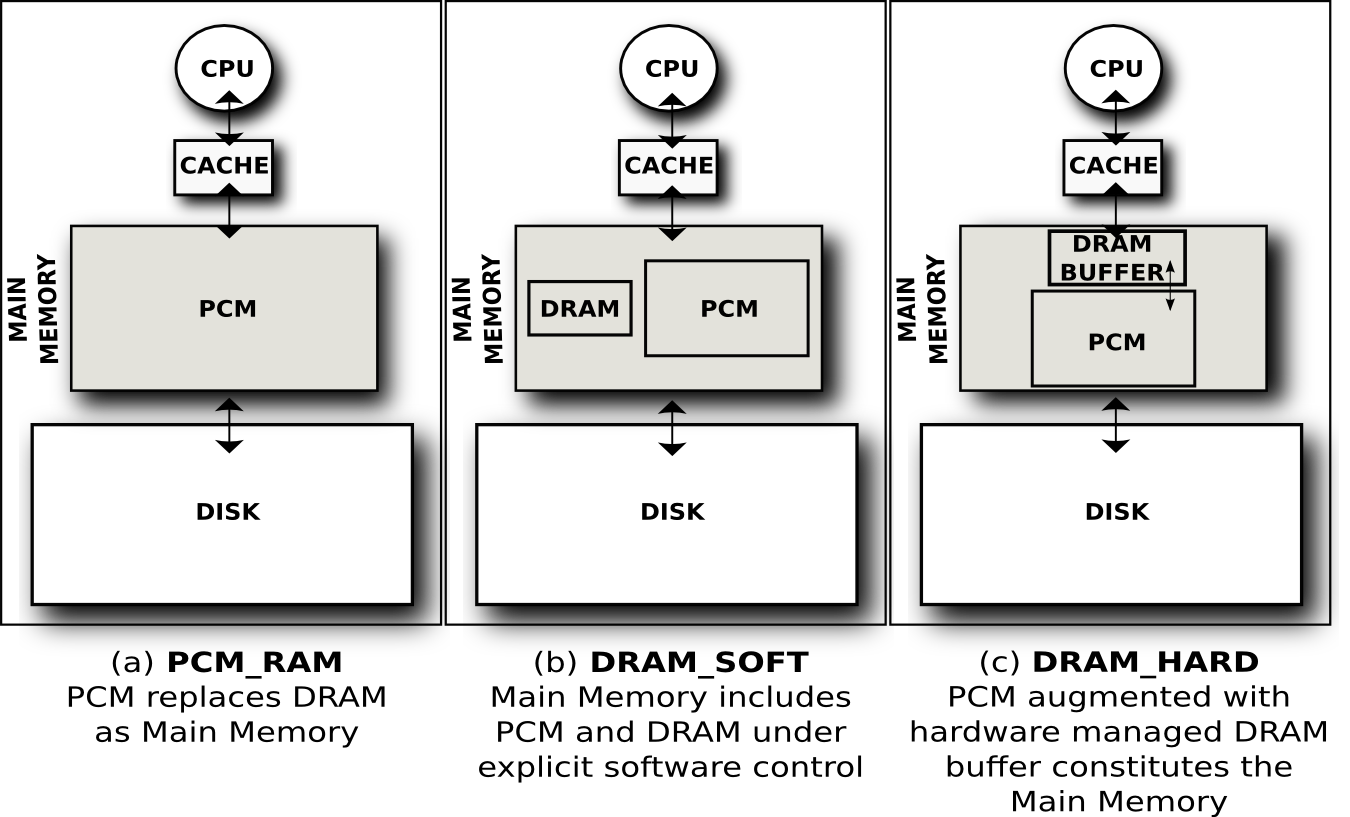
\includegraphics[height=80mm]{./fig/PCM_Models.png}\centering
	\caption{PCM-based Architectural Options \cite{chen}}
	\label{fig:pcm_models}
\end{figure}

There are several practical advantages of the \model{} configuration:
First, the write latency drawback of \modelPcmRam{} can be largely
concealed by the intermediate DRAM buffer~\cite{qureshi}. Second,
existing applications can be used \textit{as is} but still manage to take
advantage of both the DRAM and the PCM. This is in stark contrast to the
\modelExplicit{} model which requires incorporating additional machinery,
either in the program or in the OS, to distinguish between data mapped
to DRAM and to PCM -- for example, by having separate address space
mappings for the different memories.

\subsection*{Our Work}
In this paper, we propose minimalist reworkings, that are tuned to
the \model{} model,  of current implementations of database operators.
In particular, we focus on the ``workhorse'' operators:
\textit{sort}, \textit{hash join} and \textit{group-by}.
The proposed modifications are not only easy to implement but are attractive from the performance perspective also, simultaneously reducing
\emph{both} PCM writes and query response times.
The new implementations are evaluated on Multi2sim
\cite{multi2sim}, a state-of-the-art architectural simulator, after
incorporating major extensions to support modelling of the \model{}
configuration.  Their performance is evaluated on \emph{complete}
TPC-H benchmark queries. This is a noteworthy point since earlier studies
of PCM databases had only considered operator performance in isolation.
But, it is possible that optimizing a specific operator may turn out to be detrimental
to downstream operators that follow it in the query execution plan. For
instance, the proposal in \cite{chen} to keep leaf nodes unsorted in B$^+$
indexes -- while this saves on writes, it is detrimental to the running
times of \emph{subsequent} operators that leverage index ordering -- for instance, \emph{join filters}.
Finally, we include the metric of \emph{wear distribution}
in our evaluation to ensure that the reduction in writes is not achieved
at the cost of skew in wear-out of PCM cells.

Our simulation results indicate that the customized implementations
collectively offer substantive benefits with regard to PCM writes --
the number is typically brought down \emph{by a factor of two to three}.
Concurrently, the query response times are also brought down by about
\emph{20--30 percent}. As a sample case in point, for TPC-H Query 19,
savings of 64\% in PCM writes are achieved with a concomitant 32\%
reduction in CPU cycles. 

Fully leveraging the new implementations requires integration with
the query optimizer, an issue that has been largely overlooked in
the prior literature. We take a first step here by providing simple
but effective statistical \emph{estimators} for the number of writes
incurred by the new operators,
and incorporating these estimators in the query optimizer's cost model.
Sample results demonstrating that the resultant plan choices provide
substantively improved performance are provided in our experimental study.

Overall, the above outcomes augur well for the impending migration
of database engines to PCM-based computing platforms.

\subsection*{Organization}
The remainder of this paper is organized as follows: We define the
problem framework in Section~\ref{sec:framework}. The design of the new
PCM-conscious database operators, and an analysis of their PCM writes,
are presented in Sections~\ref{sort}, \ref{hj} and \ref{gby}.
Our experimental framework and the simulation results are reported in
Sections~\ref{sec:exp} and \ref{sec:results}, respectively. This is followed by a
discussion in Section~\ref{integration} on integration with the query optimizer. 
The related literature is reviewed in Section~\ref{relWork}. Finally,
Section~\ref{conclusion} summarizes our conclusions and outlines future
research avenues.

\section{Problem Framework}
\label{sec:framework}
In this section, we overview the problem framework, the assumptions made
in our analysis, and the notations used in the sequel.

We model the \model{} memory organization shown in Figure~\ref{fig:pcm_models} (c). 
The DRAM buffer is of size $D$, and organized in a \emph{K-way
set-associative} manner, like the L1/L2 processor cache memories. Moreover,
its operation is identical to that of an \emph{inclusive} cache in the
memory hierarchy, that is, a new DRAM line is fetched from PCM each time there
is a DRAM miss. The last level cache in turn fetches its data from the
DRAM buffer.

We assume that the writes to PCM are in word-sized units (4B) and are incurred only when a data block is evicted from DRAM to PCM. A \textit{data-comparison write (DCW)} scheme \cite{write} is used for
the writing of PCM memory blocks during eviction from DRAM -- in this
scheme, the memory controller compares the existing PCM block to the newly
evicted DRAM block, and selectively writes back only the modified words.
Further, \textit{N-Chance}~\cite{nchance} is used as the DRAM eviction
policy due to its preference for evicting non-dirty entries, thereby
saving on writes. The failure recovery mechanism for updates is orthogonal to our work and is therefore not discussed in this paper.

As described above, the simulator implements a realistic DRAM
buffer. However, in our write analyses and estimators, we assume for
tractability that there are no conflict misses in the DRAM. Thus, for
any operation dealing with data whose size is within the DRAM capacity,
our analysis assumes no evictions and consequently no writes. The experimental
evaluation in Section~\ref{sec:validation} indicates the 
impact of this assumption to be only marginal.

With regard to the operators, we use $R$ to denote the input relation
for the \textit{sort} and \textit{group-by} unary operators.  Whereas,
for the binary \textit{hash join} operator, $R$ is used to denote the
smaller relation, on which the hash table is constructed, while $S$
denotes the probing relation. 

In this paper, we assume that all input relations are \emph{completely PCM-resident}.
Further, for presentation simplicity, we assume that the sort,
hash join and group-by expressions are on singleton attributes --
the extension to multiple attributes is straightforward.

A summary of the main notation used in the analysis of the following
sections is provided in Table~\ref{tab:notations}.

\begin{table}[t]
\centering
\caption{Notations Used in Operator Analysis}
\label{tab:notations}
\begin{small}
\begin{tabular}{p{2cm}p{11cm}}
\toprule  
\textbf{Term} & \textbf{Description}\\ 
\midrule
\textbf{$D$} & DRAM size\\
\textbf{$K$} & DRAM Associativity\\
\textbf{$N_R, N_S$} & Row cardinalities of input relations R and S, respectively\\
\textbf{$L_R, L_S$} & Tuple lengths of input relations R and S, respectively\\
\textbf{$P$} & Pointer size\\
\textbf{$\hashsize$} & Size of each hash table entry\\
\textbf{$\aggsize$} & Size of aggregate field (for group-by operator)\\
\textbf{$\hjcount,\gbcount$} & Output tuple cardinalities of join and group-by operators, respectively\\
\textbf{$\hjlen,\gblen$} & Output tuple lengths of join and group-by operators, respectively\\
\bottomrule
\end{tabular}
\end{small}
\end{table}


\chapter{Operator Algorithms}
\section{The \emph{Sort} Operator} \label{sort}

Sorting is among the most commonly used operations in database systems, forming
the core of operators such as \emph{merge join}, \emph{order-by} and some
flavors of \emph{group-by}.  The process of sorting is quite write-intensive
since the commonly used in-memory sorting algorithms, such as
\textit{quicksort}, involve considerable data movement. In the single pivot
quicksort algorithm with $n$ elements, the average number of swaps is of the
order of $0.3nln(n)$~\cite{swaps}. There are other algorithms such as
\emph{selection sort} which involve much less data movement, but they incur
\emph{quadratic} time complexity in the number of elements to be sorted, and are
therefore unsuitable for large datasets.

The main advantage associated with the quicksort algorithm is that it has good
average-case time complexity and that it sorts the input data in-place. If the
initial array is much larger than the DRAM size, it would entail evictions from
the DRAM during the swapping process of partitioning. These evictions might lead
to PCM writes if the evicted DRAM lines are \textit{dirty}, which is likely
since elements are being swapped. If the resulting partition sizes continue to
be larger than DRAM, partitioning them in turn will again cause DRAM evictions
and consequent writes. Clearly, this trend of writes will continue in the
recursion tree until the partition sizes become small enough to fit within DRAM.
Thereafter, there would be no further evictions during swapping and the
remaining sorting process would finish inside the DRAM itself.

From the above discussion, it is clear that it would be desirable for the
sorting algorithm to converge fast to partition sizes below DRAM size with
fewer number of swaps. For uniformly-distributed data, these requirements are
satisfied by \emph{flashsort}~\cite{flashsort}. On the other hand, for data with
skewed distribution, we propose a variant of flashsort called \emph{multi-pivot
flashsort}. This algorithm adopts the pivot selection feature of the quicksort 
algorithm into flashsort in order to tackle the skewness in data.

Both these algorithms are discussed in detail in the following sections. 

\subsection{Data with uniform distribution}\label{sort_uniform} 

The flashsort algorithm can potentially form DRAM-sized partitions in a
\emph{single} partitioning step with at most $N_R$ swaps. The sorting is done
in-place with a time complexity of $O(N_Rlog_2N_R)$ with constant extra space.
The flashsort algorithm proceeds in three phases: \emph{Classification},
\emph{Permutation} and \emph{Short-range Ordering}. A brief description of each
of these phases is as follows:

\subsubsection{Classification phase} The classification phase divides the input
data into equi-range partitions comprising of contiguous and disjoint ranges.
That is, if p partitions are required (where p is an input parameter), the
difference between the minimum and the maximum input values is divided by p.
Subsequently, each tuple is mapped to a partition depending on in which range
the value of the sorting attribute of the tuple lies.  Specifically, a tuple
with attribute value $v$ is assigned to $Partition(v)$, computed as
$$Partition(v) = 1 + \lfloor \frac{(p-1)(v- v_{min})}{v_{max}-v_{min}} \rfloor$$
where $v_{min}$ and $v_{max}$ are the smallest and largest attribute values in
the array, respectively. The number of tuples in each such partition is counted
to derive the boundary information.  We choose the number of partitions $p$ to
be $\lceil c \times \frac{N_R L_R}{D} \rceil$, where $c \geq 1$ is a multiplier
to cater to the space requirements of additional data structures constructed
during sorting. In our experience, setting $c = 2$ works well in practice.

\subsubsection{Permutation phase} The Permutation phase moves the elements to
their respective partitions by leveraging the information obtained in the
Classification phase. The elements are swapped in a cyclic manner to place each
element inside its partition boundary with a single write step per element. 

\subsubsection{Short-range Ordering phase} The resulting partitions, each having
size less than $D$, are finally sorted in the Short-range Ordering phase using
quicksort. Note that, by virtue of their size, these partitions are not expected
to incur any evictions during the process of sorting.  \\

\textbf{PCM write analysis}: Though the partition boundary counters are
continuously updated during the Classification phase, they are expected to incur
very few PCM writes. This is because the updates are all in quick succession,
making it unlikely for the counters to be evicted from DRAM during the update
process. Next, while in the Permutation phase, there are no more than $N_R L_R$
writes since each tuple is written at most once while placing it inside its
partition boundaries. Since each partition is within the DRAM size, its
Short-range Ordering phase will finish in the DRAM itself, and then there will
be another $N_R L_R$ writes upon eventual eviction of sorted partitions to PCM. 

Thus, the number of word-writes incurred by this algorithm is estimated by
\begin{equation} \label{eq:sort} \FlashsortWrites = \dfrac{2N_RL_R}{4} = \dfrac{N_R
L_R}{2} \end{equation}

\subsection{Data with non-uniform distribution} \label{sort_non_uniform} 

In the case when the data is non-uniformly distributed, the equi-range
partitioning used by flashsort fails to produce equi-sized partitions. This is
because the number of tuples in each range is now dependent on the skew of the
data.  We therefore propose an alternative algorithm, called \emph{multi-pivot flashsort}, 
which uses multiple pivots
instead to partition the input tuples. These pivots are randomly-chosen from the input
itself, in the same manner as conventional quicksort selects a single pivot to
create two partitions. The chosen pivots are subsequently leveraged to partition the 
input during sorting.  

The modified phases of this alternative implementation of the flashsort algorithm, along 
with their pseudo-codes, are described next.

\subsubsection{Classification phase} In the Classification phase, we divide the
input relation into $p$ partitions, where $p = \lceil \frac{N_R L_R}{D}
\rceil$, using $p-1$ random tuples as pivots. Since the pivots are picked at
random, the hope is that each partition is approximately of size $D$.  These
pivots are then copied to a separate location and sorted. Subsequently, we scan
through the array of tuples in the relation, counting the number of elements
between each consecutive pair of pivots. This is accomplished by carrying out,
for each tuple in the array, a binary search within the sorted list of pivots.

In spite of the random choice of pivot values, it is quite possible that some
partitions may turn out to be larger than the DRAM. We account for this
possibility by conservatively creating a larger number of initial partitions.
Specifically, the number of partitions is $p = \lceil c \times \frac{N_R
L_R}{D} \rceil$, where $c \geq 1$ is a design parameter similar to the one used
in the flashsort algorithm. Subsequently, we consider each pair of adjoining
partitions and coalesce them if their total size is within the DRAM size, after
leaving some space for bookkeeping information. 

While the above heuristic approach is quite effective, it still does not
guarantee that all the resultant partitions will be less than DRAM size. The
(hopefully few) cases of larger-sized partitions are subsequently handled
during the Short-range Ordering phase.

The pseudo-code for the Classification phase is outlined in
Algorithm~\ref{alg:read_phase}.

%\begin{algorithm}
\small
\caption{Classification Phase}
\label{alg:read_phase}
\textbf{array[]} is the array of input tuples\\
\textbf{c} is a design parameter $\geq 1$\\
\begin{algorithmic}[1]
\State p = $\lceil c\times \frac{N_R L_R}{D} \rceil$
\State randIndex[] = generate $p-1$ random indexes
\State pivot[] = array[randIndex];
\State sort(pivot[])
\State size[] = {0...0}   
\Comment{size of sub-arrays}
\State partitionStart[] = {0...0}
\Comment{starting offset of each partition}
\For {i=$1$ to $N_R$}
\State partition = getPartition(array[i]) 
\State size[partition]++ 
\EndFor
\Comment {Time complexity=$N_R\times log_2p$ }
\State cumulative = 0
\For {i=$1$ to $p$}
\State cumulative = cumulative + size[i]
\State partitionStart[i+1] = cumulative
\EndFor
\Comment {Time complexity=$p$ }
\State return partitionStart[]
\end{algorithmic}

\end{algorithm}


\subsubsection{Permutation phase} The Permutation phase uses the information
gathered in the Classification phase to group tuples of the same partition
together. A slight difference from flashsort here is that the attribute value
now needs to be compared against the sorted list of pivots to determine the
partition of the tuple.  The pseudo-code for the Permutation phase is shown in
Algorithm~\ref{alg:swap_phase}.  The maximum number of writes is bounded by
$N_R L_R$, corresponding to the worst case where \emph{every} tuple has to be
moved to its correct partition.

%\begin{algorithm}[h!]
\small
\caption{Permutation Phase}
\label{alg:swap_phase}
\textbf{partitionStart[]} is obtained from Classification Phase\\
\textbf{nextUnresolvedIndex[]} indicates the next position to be examined for each partition\\
\begin{algorithmic}[1]
\State nextUnresolvedIndex[] = partitionStart[]
\For {i=1 to $N_R$}
	\State curPartitionCorrect = getPartition(array[i])
     \If {i between partitionStart[curPartitionCorrect] and  partitionStart[curPartitionCorrect+1]}                
     \State nextUnresolvedIndex[curPartitionCorrect] = i+1
	\State continue
     \Else
     		\State firstCandidateLoc = i
			\State presentCandidate = array[i]             
            \State flag = 1
            \While {flag} 
                \State targetPartitionStart = nextUnresolvedIndex[curPartitionCorrect]
                \State targetPartitionEnd = partitionStart[curPartitionCorrect + 1]
                \For {k=targetPartitionStart to targetPartitionEnd} 
                \State nextPartitionCorrect = getPartition(array[i])
                    \If {k between partitionStart[nextPartitionCorrect]                       and 
                    \State partitionStart[nextPartitionCorrect + 1]}
                        \State continue
                        
                    \ElsIf {k == firstCandidateLoc} 
                        \State flag = 0 \Comment Indicates it is a cycle
                    \EndIf
                    \State swap(presentCandidate, array[k])
                    \State nextUnresolvedIndex[curPartitionCorrect] = k+1
                    \State curPartitionCorrect = nextPartitionCorrect
                    
                    \State break
             
				\EndFor
			\EndWhile
	\EndIf
\EndFor
\Comment {Time complexity=$N_R\times log_2p$ }
\end{algorithmic}

\end{algorithm}

\subsubsection{Short-range Ordering phase} Finally, each of the partitions are
sorted separately using conventional quicksort to get the final PCM sorted
array. For partitions that turn out to be within the DRAM size, the Short-range
Ordering phase is completed using conventional quicksort. On the other hand, if some
larger-sized partitions still remain, we recursively apply the multi-pivot
flashsort algorithm to sort them until all the resulting partitions can fit inside
DRAM and can be internally sorted.

%\begin{algorithm}
\small
\caption{Short-range Ordering Phase}
\label{alg:sort_phase}
\begin{algorithmic}[1]
\For {i=1 to p}
\If {size[p] $<$ D}
\State quicksort (partition p)
\Else 
\State multi-pivot flashsort (partition p)
\EndIf 
\EndFor
\end{algorithmic}

\end{algorithm}

Figure~\ref{fig:mpsort} visually displays the steps involved in the multi-pivot
flashsort of an array of nine values. First, in the Classification phase, $30$
and $10$ are randomly chosen as the pivots. These pivots divide the input
elements into 3 different ranges: ($< 10$), ($\geq 10$, $< 30$), ($\geq 30$).
The count of elements in each of these ranges is then determined by making a
pass over the entire array -- in the example shown, three elements are present
in each partition.  Then, in the Permutation phase, the elements are moved to
within the boundaries of their respective partitions. Finally, in the
Short-range Ordering phase, each partition is separately sorted within the
DRAM.

%\begin{figure}[h]
%	\centering
%	\subfloat[Classification Phase]{	
%  	\includegraphics[width=8cm]{sort_step_1.png}
%  	
%  	\begin{tabular}{|c|c|c|y|c|y|c|c|c|}
%        \hline
%        12&3&33&30&11&10&7&32&8\\\hline
%    \end{tabular}
%    }
%	\hspace{0mm}
%	\subfloat[Permutation Phase]{
%  	\begin{tabular}{|x|x|x|y|y|y|z|z|z|}
%        \hline
%        7&3&8&12&11&10&30&32&33\\\hline
%    \end{tabular}
%    }
%    \hspace{0mm}
%	\subfloat[Short-range Ordering Phase]{
%  	\begin{tabular}{|x|x|x|y|y|y|z|z|z|}
%        \hline
%        3&7&8&10&11&12&30&32&33\\\hline
%    \end{tabular}
%    }
%	\caption{Multi-Pivot Flashsort}
%	\label{fig:mpsort}
%	
%\end{figure}

%\newcolumntype{b}{>{\columncolor{white}}c}
\textbf{PCM write analysis}: The analysis follows that of the flashsort
algorithm. A negligible number of writes would be incurred during the copying and
sorting of the pivots. As mentioned, the writes during Permutation phase would 
be below $N_R L_R$. The creation of additional partitions by choosing extra
pivots, and their subsequent coalescing, increases the likelihood that each
partition is below DRAM size--akin to that in flashsort. Therefore
the total word-writes is again estimated to be \begin{equation}
\label{eq:mpivot} \MPFlashsortWrites = \frac{N_RL_R}{2} \end{equation}

\section{The \emph{Hash Join} Operator}
\label{hj}
Hash join is perhaps the most commonly used join algorithm in database
systems. Here, a hash table is built on the smaller relation, and tuples
from the larger relation are used to probe for matching values in the join
column. Since we assume that all tables are completely PCM-resident, the
join here \emph{does not} require any initial partitioning stage. Instead,
we directly proceed to the join phase. Thus, during the progress of hash join, writes will be incurred during the building of the hash table,
and also during the writing of the join results.

Each entry in the hash table consists of a pointer to the corresponding
build tuple, and the hash value for the join column. Due to the
absence of prior knowledge about the distribution of join column values
for the build relation, the hash table is expanded dynamically according
to the input. Typically, for each insertion in a bucket, a new space is
allocated, and connected to existing entries using a pointer. Thus,
such an approach incurs an additional pointer write each time a new
entry is inserted.

Our first modification is to use a well-known technique of allocating
space to hash buckets in units of \textit{pages} \cite{paging}. A
page is of fixed size and contains a sequence of contiguous fixed-size
hash-entries.  When a page overflows, a new page is allocated and linked to
the overflowing page via a pointer.  Thus, unlike the conventional hash
table wherein each \emph{pair} of entries is connected using pointers,
the interconnecting pointer here is only at page granularity. Note that
although open-addressing is another alternative for avoiding pointers,
probing for a join attribute value would have to search through the
\emph{entire table} each time, since the inner table may contain
\emph{multiple} tuples with the same join attribute value.

A control bitmap is used to indicate whether each entry in a page is vacant
or occupied, information that is required during both insertion and search in the
hash table. Each time a bucket runs out of space, a new page is allocated
to the bucket. Though such an approach may lead to space wastage when
some of the pages are not fully occupied, we save on the numerous pointer
writes that are otherwise incurred when space is allocated on a per-entry basis.

Secondly, we can reduce the writes incurred due to storing of the hash values in
the hash table by restricting the length of each hash value to just a single byte. In this
manner, we trade-off precision for fewer writes. If the hash function
distributes the values in each bucket in a perfectly uniform manner, it
would be able to distinguish between $2^8 = 256$ join column values in a
bucket. This would be sufficient if the number of distinct values mapping
to each bucket turn out to be less than this value. Otherwise, we would
have to incur the penalty (in terms of latency) of reading the actual join
column values from PCM due to the possibility of false positives.

\begin{figure}[htpb]
	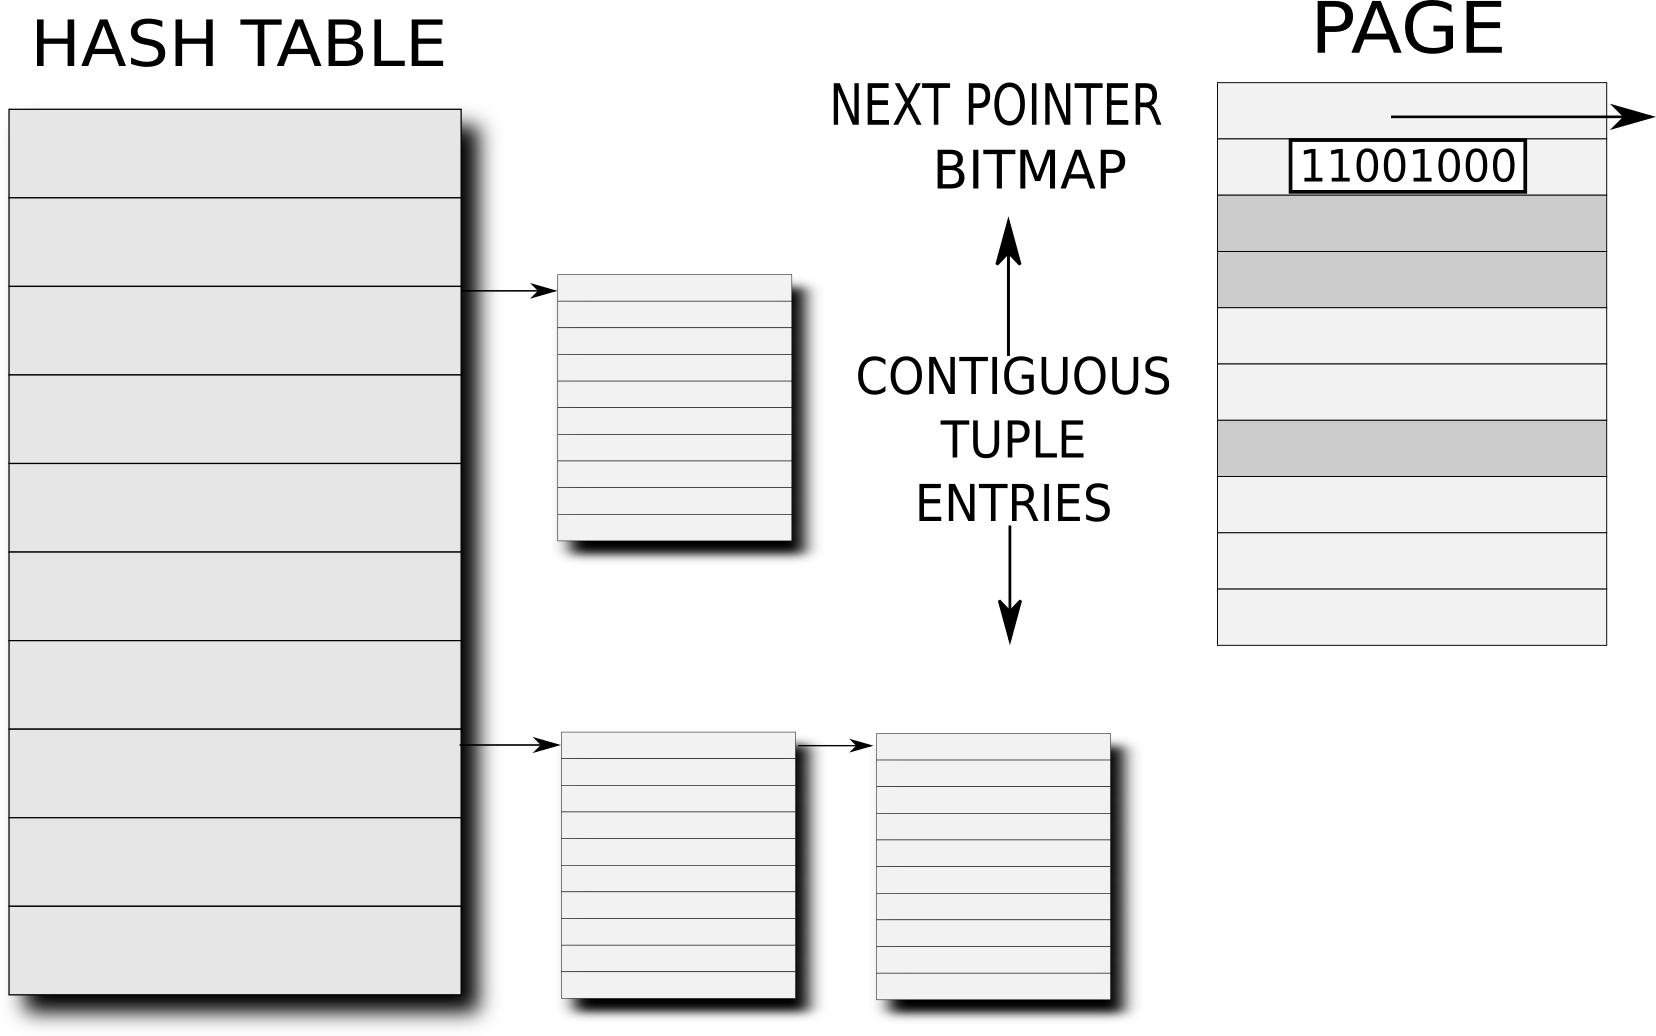
\includegraphics[height=80mm]{./fig/hash_table.png}\centering
	\caption{Paged Hash Table}
	\label{fig:hash_table}
\end{figure}

Figure~\ref{fig:hash_table} displays the hash table organization with the proposed optimizations.

\textbf{PCM write analysis}: We ignore the writes incurred while initializing each hash table bucket since they are negligible in comparison to inserting the actual entries. Assuming there are $E_{page}$ entries per page, there would now be one pointer for each $E_{page}$ set of entries. Additionally, for each insertion, a bit write would be incurred due to the bitmap update. The join tuples would also incur writes to the tune of $\hjcount \times \hjlen$. Thus, the total number of word-writes for hash join would be
$$W_{hj} = \frac{N_R \times (\hashsize +  \frac{P}{E_{page}} + \frac{1}{8} ) + \hjcount \times \hjlen }{4}$$
Since in practice both  $\frac{P}{E_{page}}$ and $\frac{1}{8}$ are small as compared to $\hashsize$, 
\vspace{-0.05in}
\begin{equation}\label{eq:hj}
 W_{hj} \approx \frac{ N_R \times \hashsize + \hjcount \times \hjlen}{4} 
\end{equation} 

\section{The \emph{Group-By} Operator}%
\label{gby}
We now turn our attention to the group-by operator which typically
forms the basis for aggregate function computations in SQL queries.
Common methods for implementing group-by include \textit{sorting} and
\textit{hashing} -- the specific choice of method depends both on the
constraints associated with the operator expression itself, as well as
on the downstream operators in the plan tree. We discuss below the
PCM-conscious modifications of both implementations, which share
a common number of \emph{output} tuple writes, namely $\gbcount \times \gblen$.

\subsection{Hash-Based Grouping}

A hash table entry for group-by, as compared to the corresponding
entry in hash join, has an additional field containing the aggregate
value. For each new tuple in the input array, a bucket index is
obtained after hashing the value of the column present in the group-by
expression. Subsequently, a search is made in the bucket indicated by
the index. If a tuple matching the group-by column value is found, the
aggregate field value is updated; else, a new entry is created in the
bucket. Thus, unlike hash join, where each build tuple had its individual
entry, here the grouped tuples share a common entry with an aggregate
field that is constantly updated over the course of the algorithm.

Since the hash table construction for group-by is identical to that
of the hash join operator, the PCM-related modifications described
in Section~\ref{hj} can be applied here as well. That is, we employ
a page-based hash table organization, and a reduced hash value size,
to reduce the writes to PCM.

\textbf{PCM write analysis}: From the above discussion, it is easy to see
that the total number of word-writes incurred for the PCM-conscious hash-based group-by is given by
\begin{equation}
\label{eq:gb_ht}
W_{gb\_ht} = \frac {\gbcount \times \hashsize + 
N_R \times \aggsize + \gbcount \times \gblen}{4}
\end{equation}

\subsection{Sort-Based Grouping}

Sorting may be used for group-by when a fully ordered operator such
as \textit{order by} or \textit{merge join} appears downstream in the plan
tree. Another use case is for queries with a \textit{distinct} clause
in the aggregate expression, in order to identify the duplicates that have
to be discarded from the aggregate.  

Sorting-based group-by differs in a key aspect from sorting itself
in that the sorted tuples do not have to be written out. Instead, it
is the aggregated tuples that are finally passed on to the next operator
in the plan tree. Hence, we can modify the flashsort algorithm of
Section~\ref{sort} to use \emph{pointers} in both the
Permutation and Short-range Ordering phases, subsequently leveraging these
pointers to perform aggregation on the sorted tuples. 

\textbf{PCM write analysis}: The full tuple writes of $2 N_R L_R$
which were incurred in the flashsort scheme, are
now replaced by $2N_R \times P$ since pointers are used during
both the Classification and Short-range Ordering phases. Thus, the total number of word-writes for this
algorithm for uniformly distributed data would be
\begin{equation}
\label{eq:gb_sort}
W_{gb\_sort} = \frac{2N_R \times P + \gbcount \times \gblen}{4}
\end{equation}


\chapter{Experimental Evaluation}
\section{Simulation Testbed}
\label{sec:exp}

This section details our experimental settings in terms of the hardware
parameters, the database and query workload, and the performance metrics
on which we evaluated the PCM-conscious operator implementations.



\subsection{Architectural Platform}
Since PCM memory is as yet not commercially available, we
have taken recourse to a simulated hardware environment to
evaluate the impact of the PCM-conscious operators.  For this
purpose, we chose Multi2sim~\cite{multi2sim}, an open-source
application-only\footnote{Simulates only the application layer without
the OS stack.} simulator.

\begin{center}
\begin{table}[h]
\begin{small}
\caption{Experimental Setup}
\label{table:setup}
\begin{tabular}{p{4cm}p{12cm}}
\toprule
Simulator & Multi2sim-4.2 with added support for PCM\\ \hline

L1D cache (private) & 32KB, 64B line, 4-way set-associative, 4 cycle latency, write-back, LRU\\ \hline
L1I cache (private) & 32KB, 64B line, 4-way set-associative, 4 cycle latency, write-back, LRU\\ \hline   
L2 cache (private) & 256KB, 64B line, 4-way set-associative, 11 cycle latency, write-back, LRU\\ \hline

DRAM buffer (private) & 4MB, 256B line, 8-way set-associative, 200 cycle latency, write-back, N-Chance (N = 4)\\ \hline

Main Memory & 2GB PCM, 4KB page, 1024 cycle read latency (per 256B line), 64 cycle write latency (per 4B modified word)\\ \bottomrule
\end{tabular}
\end{small}
\end{table}
\end{center}

We evaluated the algorithms on Multi2sim in cycle-accurate simulation
mode. Since it does not have native support for PCM, we made a major
extension to its existing memory module to model PCM memory. Specifically,
the following enhancements were incorporated in the simulator to conduct
our experimental evaluation:

\textbf{Hybrid Main Memory}: 
The memory organization was extended such that the new configuration
consists of PCM with a hardware controlled DRAM buffer. The DRAM buffer
acts as another level of cache in the memory hierarchy, specifically
between the L2 cache and the PCM.

\textbf{New DRAM Replacement Policy}: 
The DRAM is simulated as a set-associative write-back memory with
\textit{N-Chance} as the eviction policy. As mentioned in \cite{nchance},
$N$ was set to $\frac{K}{2}$, where $K$ is the cache associativity,
since this setting was found to provide good performance on multiple
metrics -- writes, energy and latency.

\textbf{Tracking DRAM-PCM Data}:
Like most other architectural simulators, Multi2sim does not explicitly
track the data residing at the different levels of the memory
hierarchy. It instead maintains only a single buffer that indicates
the latest data, as visible to the simulated program, for each memory
location. We therefore had to add separate data tracking functionality
for the DRAM and PCM resident data.

\textbf{Data Comparison Write Scheme}: 
The write-back mechanism of data from DRAM to PCM was modelled on the
DCW~\cite{write} scheme. Thus, for each evicted DRAM block, a comparison
to the original PCM resident data block was made, and writes were
restricted to only those words where the data bits differed. In our
experiments, we measured writes at \textit{word} (4B) granularity.

\textbf{Asymmetric Read-Write Latencies}:  
The timing simulation was modified to account for the higher write
latency of PCM as compared to a read.

\textbf{Wear Distribution}: 
Apart from the raw number of writes, a critical related metric for PCM
algorithms is their wear distribution. We therefore instrumented the
Multi2sim code to track block level wear distribution information. To
achieve this, separate counters were created that tracked writes to each
PCM \textit{line} (256B) during the query processing activity.

\textbf{Intermediate Statistics}: 
Multi2sim does not have support to track intermediate statistics during
a program run. We therefore provided additional inter-process communication capabilities in the
tool so that the simulated program could ask the simulator to dump
statistics for each intermediate operator during the execution of a query.


The specific configurations of the memory hierarchy \emph{(L1 Data,
L1 Instruction, L2, DRAM Buffer, PCM)} used for evaluation in our experiments are
enumerated in Table~\ref{table:setup}.  These values are scaled-down
versions, w.r.t. number of lines, of the hardware simulation parameters used
in \cite{wear} -- the reason for the scaling-down is to ensure that the
simulator running times are not impractically long. However, we have been
careful to ensure that the \emph{ratios} between the capacities of adjacent
levels in the hierarchy are maintained as per the original configurations
in \cite{wear}.  

%\vspace*{0.05in}

\subsection{Database and Queries}
%We used TPC-H (version 2.16.0) 1GB PCM-resident database for our experiments.
For the data, we used the default 1GB database generated by the
TPC-H \cite{tpch} benchmark.  This size is certainly very small compared to the
database sizes typically encountered in modern applications -- however,
we again chose this reduced value to ensure viable simulation running
times. Furthermore, the database is significantly larger than the
simulated DRAM (4MB), representative of most real-world
scenarios.

For simulating our suite of database operators -- \textit{sort},
\textit{hash join} and \textit{group-by} -- we created a separate library
consisting of their native PostgreSQL \cite{postgres} implementations. To
this library, we added the PCM-conscious versions described in the
previous sections.

While we experimented with several of the TPC-H queries, results for
three queries: {\sf Query 13 (Q13)}, {\sf Query 16 (Q16)} and {\sf Query 19 (Q19)}, that
cover a diverse spectrum of the experimental space, are presented here.
For each of the queries, we first identified the execution plan
recommended by the PostgreSQL query optimizer with the native operators,
and then forcibly used the same execution plan for their PCM-conscious
replacements as well. This was done in order to maintain fairness in the
comparison of the PCM-oblivious and PCM-conscious algorithms, though it
is possible that a \emph{better} plan is available for the PCM-conscious
configuration -- we return to this issue 
later in Section~\ref{integration}.  The execution plans associated with the
three queries are shown in Figure~\ref{fig:plan_trees}. 
 


\begin{figure*}[t]
\centering
\subfloat[Q13]{
\begin{tikzpicture}[scale=.75, transform shape]

\tikzstyle{every node} = [rectangle, fill=gray!5]

\node (d) at (0,3) {Index Scan / Filter};
\node (c) at (0,1.5) {CUSTOMER};

\node (s) at (3,3) {Sort};
\node (p) at (3,2.25) {Seq. Scan / Filter};
\node (a) at (3,1.5) {ORDERS};

\node (e) at (1.5,4) {Merge Left Join};
\node (f) at (1.5,5)  {Group Aggregate};
\node (g) at (1.5,6)  {Hash Aggregate};
\node (h) at (1.5,7)  {Sort};


\draw[-] (c) -- (d);
\draw[-] (a) -- (p);
\draw[-] (d) -- (e);
\draw[-] (p) -- (s);
\draw[-] (s) -- (e);
\draw[-] (e) -- (f);

\draw[-] (f) -- (g);
\draw[-] (g) -- (h);

\end{tikzpicture}
}
\subfloat[Q16]{
\begin{tikzpicture}[scale=.75, transform shape]

\tikzstyle{every node} = [rectangle, fill=gray!5]

\node (d) at (0,3) {Seq. Scan / Filter};
\node (c) at (0,1.5) {PARTSUPP};

\node (s) at (3,3) {Hash};
\node (p) at (3,2.25) {Seq. Scan / Filter};
\node (a) at (3,1.5) {SUPPLIER};

\node (e) at (1.5,4) {Hash Anti Join};

\node (n) at (5.5, 4) {Hash};
\node (b) at (5.5,3) {Seq. Scan / Filter};
\node (x) at (5.5,1.5) {PART};

\node (f) at (2.5,5)  {Hash Join};
\node (g) at (2.5,6)  {Group Aggregate};
\node (h) at (2.5,7)  {Sort};


\draw[-] (c) -- (d);
\draw[-] (a) -- (p);
\draw[-] (d) -- (e);
\draw[-] (p) -- (s);
\draw[-] (s) -- (e);
\draw[-] (e) -- (f);

\draw[-] (x) -- (b);
\draw[-] (b) -- (n);
\draw[-] (n) -- (f);

\draw[-] (f) -- (g);
\draw[-] (g) -- (h);

\end{tikzpicture}

}
\subfloat[Q19]{


\begin{tikzpicture}[scale=.75, transform shape]

\tikzstyle{every node} = [rectangle, fill=gray!5]

\node (d) at (0,3.5) {Index Scan / Filter};
\node (c) at (0,1.5) {PART};

\node (s) at (3,3.5) {Hash};
\node (p) at (3,2.5) {Seq. Scan / Filter};
\node (a) at (3,1.5) {LINEITEM};

\node (e) at (1.5,5) {Hash Join};
\node (f) at (1.5,7)  {Aggregate};


\draw[-] (c) -- (d);
\draw[-] (a) -- (p);
\draw[-] (d) -- (e);
\draw[-] (p) -- (s);
\draw[-] (s) -- (e);
\draw[-] (e) -- (f);
\end{tikzpicture}
}

\caption{ Query execution plan trees}

\label{fig:plan_trees}

\end{figure*}




\subsection{Performance Metrics}
We measured the following performance metrics for each of the queries:
\begin{description}


\item [PCM Writes:] The total number of word (4B) updates that are applied to the PCM memory during
the query execution.
\item [CPU Cycles:] The total number of CPU cycles required to execute the query.
\item [Wear Distribution:] The frequency distribution of writes measured on a per-256B-block basis.

\end{description}

\section{Experimental Results}
\label{sec:results}
Based on the above framework, we conducted a wide variety of experiments
and present a representative set of results here.  We begin by profiling the
PCM writes and CPU cycles behavior of
the native and PCM-conscious executions for Q13, Q16 and Q19 --
these results are shown in Figure~\ref{fig:overall_results}.  In addition to
the standard TPC-H
with uniform data distribution, we also show results for the sort operator
implementation on a skewed version of TPC-H, generated using a Zipfian distribution
\cite{vivekn} with a skew factor of $Z=1$. In each of these figures,
we provide
both the total and the break-ups on a per-operator basis, with \emph{GB} and
\emph{HJ} labels
denoting group-by and hash join operators, respectively.


\begin{figure*}[htpb]

\centering

\subfloat[Q13 Performance]{
  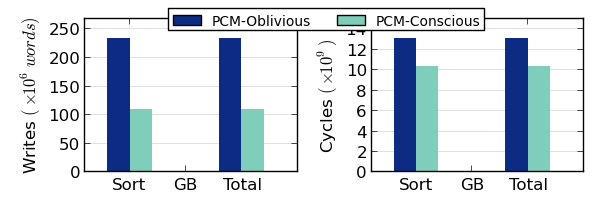
\includegraphics[height=45mm]{./fig/overall_q13.png}
  
}
%\hspace{0mm}
%\subfloat[Q13 Performance (skewed TPC-H)]{
%  \includegraphics[height=45mm]{./fig/overall_q13_skewed.png}
%  
%}
\hspace{0mm}
\subfloat[Q16 Performance]{
  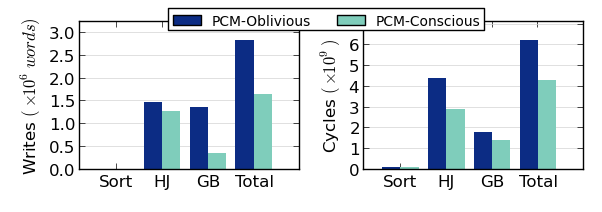
\includegraphics[height=45mm]{./fig/overall_q16.png}
}
\hspace{0mm}
\subfloat[Q19 Performance]{
  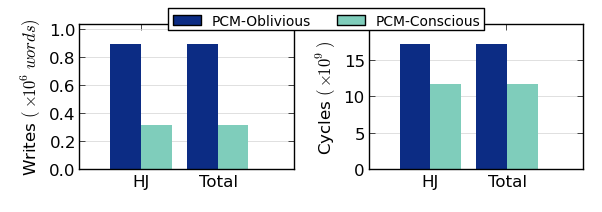
\includegraphics[height=45mm]{./fig/overall_q19.png}
}
\caption{Performance of TPC-H queries}
\label{fig:overall_results}
\end{figure*}


Focusing our attention first on Q13 in
Figure~\ref{fig:overall_results}(a), we find that the bulk of the
overall writes and cycles are consumed by the sort operator. Comparing
the performance of the Native (blue bar) and PCM-conscious (green bar)
implementations, we observe a very significant savings (53\%) on writes,
and an appreciable decrease (20\%) on cycles. For Q13 execution on skewed 
TPC-H, for which we used the multi-pivot flashsort algorithm, 
the corresponding performance numbers (Figure~\ref{fig:overall_results}(b)) are
comparatively lesser. Specifically, savings of 
44\% and 14\%  are observed in writes and cycles, respectively.

Turning our attention to Q16 in Figure~\ref{fig:overall_results}(c),
we find that here it is the group-by operator that primarily influences
the overall writes performance, whereas the hash join determines the
cycles behavior. Again, there are substantial savings in both writes
(40\%) and  cycles (30\%) delivered by the PCM-conscious approach.

Finally, moving on to Q19 in Figure~\ref{fig:overall_results}(d),
where hash join is essentially the only operator, the
savings are around $64\%$ with regard to writes and $32\%$ in cycles.

\subsection{Operator-wise Analysis}
We now analyse the savings due to each operator independently and show
their correspondence to the analyses in Sections~\ref{sort}--\ref{gby} .

\paragraph{Sort.}
For Q13 execution on uniform TPC-H, as already mentioned, we observed 
savings of $53\%$ in writes and $20\%$ in cycles. Similarly, on skewed TPC-H, these  
figures were $44\%$ (writes) and $14\%$ (cycles). 
In the case of Q16, the data at the sorting stage was
found to be much less than the DRAM size. Hence, both the native and
PCM-conscious executions used the standard sort routine, and as a result,
the cycles and writes for both implementations match exactly.

\paragraph{Hash Join.}
Each entry in the hash table consisted of a pointer to the build tuple
and a hash value field. New memory allocation to each bucket was done
in units of pages, with each page holding up to 64 entries. A search for
the matching join column began with the first tuple in the corresponding
bucket, and went on till the last tuple in that bucket, simultaneously
writing out the join tuples for successful matches.  For Q16, we
observed a $12\%$ improvement in writes and $31\%$ in cycles due to the
PCM-conscious hash join, as shown in Figure~\ref{fig:overall_results}(c). The
high savings in cycles was the result of the caching effect due to page-wise
allocation.
These improvements were even higher with Q19  -- specifically, 65\% writes and 32\%
cycles, as shown in Figure~\ref{fig:overall_results}(d). The source of the
enhancement was the 3 bytes of writes saved due to single-byte hash
values\footnote{The hash values of all entries within a bucket are placed
contiguously.}, and additionally, the page-based aggregation of hash table
entries.


\paragraph{Group-By.}
In Q16, the aggregate operator in the group-by has an associated
\textit{distinct} clause.  Thus, our group-by algorithm utilized
sort-based grouping to carry out the
aggregation. Both the partitioning and sorting were carried out through
pointers, thereby reducing the writes significantly. Consequently,
we obtain savings of $74\%$ in writes and $20\%$ in cycles, as shown
in Figure~\ref{fig:overall_results}(c).  When we consider Q13, however,
the grouping algorithm employed was hash-based. Here, the hash table consisted
of very few entries which led to the overhead of the page metadata construction
overshadowing the
savings obtained in other aspects. Specifically, only marginal improvements
of about 4\% and 1\% were obtained for writes and cycles, as shown in
Figure~\ref{fig:overall_results}(a).




\subsection{Lifetime Analysis}

The above experiments have shown that PCM-conscious operators
can certainly provide substantive improvements in both writes and
cycles. However, the question still remains as to whether these
improvements have been purchased at the expense of \emph{longevity} of
the memory. That is, are the writes skewed towards particular memory
locations?  To answer this, we show in Figure~\ref{fig:wear_dist}, the
maximum number of writes across all memory blocks for the three TPC-H queries
(as mentioned earlier,
we track writes at the block-level--256 bytes--in our modified simulator). The
x-axis displays the block numbers in 
decreasing order of writes. 

\begin{figure*}[htpb]
\centering

\subfloat[Q13]{
  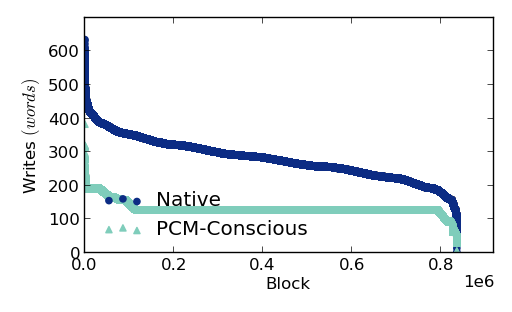
\includegraphics[width=11cm]{./fig/wear_q13.png}
}
\hspace{0mm}

\subfloat[Q16]{
  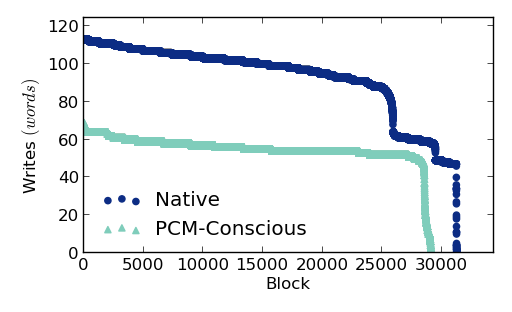
\includegraphics[width=11cm]{./fig/wear_q16.png}
}
\hspace{0mm}

\subfloat[Q19]{
  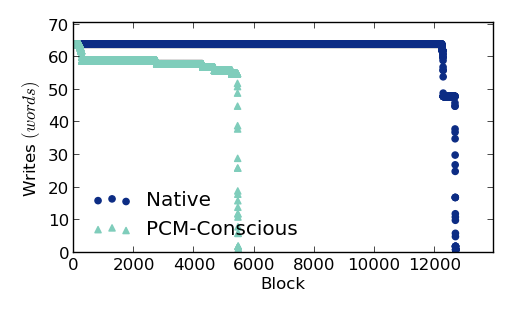
\includegraphics[width=11cm]{./fig/wear_q19.png}
}
\caption{Queries wear distribution }
\label{fig:wear_dist}
\end{figure*}


We observe here that the maximum number of writes is considerably more for the
native systems as compared to the PCM-conscious processing. This
conclusively demonstrates that the improvement is with regard to
\emph{both} average-case and worst-case behavior.

\subsection{Validating Write Estimators}
\label{sec:validation}

We now move on to validating the estimators
(presented in Sections~\ref{sort} through \ref{gby})  for the number of
writes incurred by the various database operators.

\subsubsection{Sort}
The size of the $orders$ table is approximately $214$ MB. 
The flashsort algorithm incurred writes of $110.6$M. On the other hand,
the writes for multi-pivot flashsort algorithm were $112.1$M.
Replacing the values for $N_R L_R$ with the table size in Equation~\ref{eq:sort},
we get the writes as 
$\FlashsortWrites = \MPFlashsortWrites = (214 \times 10^6)/2 = 107$M.
\noindent
Thus the estimate is close to the number of observed word-writes.



\subsubsection{Hash Join}
For the hash join in Q19, the values of $N_R$, $\hashsize$, $\hjcount$,
$\hjlen$ are $0.2$M, $5$ bytes, $120$ and $8$ bytes, respectively. 
Substituting the parameter values in Equation~\ref{eq:hj}, the writes are given by:  
$W_{hj} = (0.2 \times 10^6 \times 5  + 120 \times 8)/4  \approx 0.25$M 
\noindent
which is close to the actual word-writes of $0.32$M.

  
\subsubsection{Group-By}
The values of the parameters $N_R$, $L_R$, $P$, $\gbcount$ and $\gblen$ for Q16
are $119056$, $48$ bytes, $4$ bytes, $18341$ and $48$ bytes, respectively.  
The grouping algorithm used was sort-based grouping. Using Equation~\ref{eq:gb_sort} results in:
$W_{gb\_sort} = (2 \times 119056 \times 4 \  + 18341 \times 48)/4 = 0.46$M. 
\noindent
This closely corresponds to the observed word-writes of $0.36$M.
\\

A summary of the above results is provided in
Table~\ref{tab:estimator_validation}. It is clear that our estimators
predict the write cardinality with an acceptable degree of accuracy for
the PCM-conscious implementations, making them suitable for incorporation
in the query optimizer.

\begin{table}[!h]                                                                                       
\centering                                                                                              
\caption{Validation of Write Estimators}
  \label{tab:estimator_validation}                                                                                
  %\centering                                                                                             
  \begin{small}                                                                                           
  \begin{tabular}{p{3.5cm} c c c}
  \toprule                                                                                                
  
  \textbf{Operator} &  \textbf{Estimated Word-Writes} \;  & \textbf{Observed Word-Writes}  \; & \textbf{Error Factor} \\
                    & \textbf{(in millions)} $(e)$ & \textbf{(in millions)} $(o)$  & $(\frac{e-o}{o})$\\
  \midrule                                                                                                
  
    \textbf{Sort (uniform)} &  107 & 110.6 &  -0.03\\ 
    \textbf{Sort (non-uniform)} &  107 & 112.1 & -0.05\\ 
  \textbf{Hash Join} &  0.25 & 0.32 & -0.22\\ 
  \textbf{Group-By} &  0.46 & 0.36 & 0.27\\ 
  
  \bottomrule                                                                                             
  \end{tabular}                                                                                           
  \end{small}                                                                                             
  \end{table} 

\input{src/validation}

\chapter{Optimizer Integration}
\documentclass{article}
 \usepackage{times,alltt,xspace}
 \usepackage{epsfig,subfig,graphicx}
 \usepackage{algorithm}
 \usepackage{algpseudocode}
 \usepackage{amsmath,amsfonts,amstext,amssymb,textcomp}
 \usepackage{multicol}
 %\usepackage{enumitem}
 \usepackage{url}
 \newtheorem{lemma}{Lemma}
 \newtheorem{theorem}{Theorem}
 \newtheorem{conjecture}{Conjecture}
 \newtheorem{corollary}{Corollary}
 \newtheorem{proof}{Proof}
 \usepackage{setspace}
 \usepackage{txfonts}
 \usepackage{xcolor,colortbl}
 \usepackage{booktabs}
 \usepackage{tikz}
 \usepackage[]{caption, subfig}

\begin{document}

\section{Query Optimizer Integration} \label{integration}

In the earlier sections, given a user query, the modified operator
implementations were used for the \emph{standard} plan choice of the PostgreSQL
optimizer. That is, while the execution engine was PCM-conscious, the presence
of PCM was completely \emph{opaque} to the optimizer.  However, given the
read-write asymmetry of PCM in terms of both latency and wear factor, it is
possible that alternative plans, capable of providing better performance
profiles, may exist in the plan search space. To discover such plans, the
database query optimizer needs to incorporate PCM awareness in both the
operator cost models and the plan enumeration algorithms.

Current query optimizers typically choose plans using a latency-based costing
mechanism. We revise these models to account for the additional latency
incurred during writes. Additionally, we introduce a new metric of \emph{write
cost} in the operator cost model, representing the incurred writes for a plan
in the PCM environment, using the estimators described in Sections~\ref{sort}
to \ref{gby}.  We henceforth refer to the latency cost and the write cost of a
plan as {\bf LC} and {\bf WC}, respectively.

A new user-defined parameter, called the \emph{latency slack}, is incorporated
in the query optimizer.  This slack, denoted by $\lambda$, represents the
maximum relative slowdown, compared to the LC-optimal query plan, that is
acceptable to the user in lieu of getting better write performance.
Specifically, if the LC of the LC-optimal execution plan $P_o$ is $C_o$ and the
LC of an alternate plan $P_i$ is $C_i$, the user is willing to accept $P_i$ as
the final execution plan if $C_i \le (1+\lambda) C_o$. The $P_i$ with the least
WC satisfying this equation is considered the WC-optimal plan.

With the new metric in place, we need to revise the plan enumeration process
during the planning phase. This is because the native optimizer propagates only
the LC-optimal (and interesting order) plans through the internal nodes of the
dynamic programming lattice, which may lead to pruning of potential WC-optimal
plans. On the other hand, propagating the \emph{entire} list of sub-plans at
each internal node can end up in an exponential blow-up of the search space.  

We examined the nature of WC-optimal plans--by picking them out after
exhaustively enumerating all possible plans--for queries in the TPC-H
benchmark.  In all the experiments, we observed that the WC-optimal plan
invariably had the same \emph{join order} as the LC-optimal plan, albeit with
different operator algorithms. 
%An intuitive explanation of this observation is that join order chosen in the
%LC-optimal plan was picked up because it involved lesser data processing.
%Using a different join order then would translate to more data and
%consequently more writes.

%As an intermediate option between these two extremes, we use a heuristic
%propagation mechanism at each internal node, employing an algorithmic
%parameter, \emph{local threshold} $\lambda_l$ ($\ge\lambda$). Specifically,
%let $p_i$ and $p_o$ be a generic sub-plan and the LC-optimal sub-plan at a
%node, respectively, with $c_i$ and $c_o$ being their corresponding LC values.
%Now, along with the LC-optimal and interesting order sub-plans, we also
%propagate $p_i$ with the \emph{least} WC that satisfies $c_i \le (1+\lambda_l)
%c_o$. We observed that setting $\lambda_l = \lambda$ delivered reasonably good
%results in this respect.


%With the new metric in place, we need to revise the plan enumeration process
%during the planning phase. This is because the native optimizer propagates
%just the LC-optimal (and interesting order plans) through the internal nodes
%of the dynamic programming lattice, which may lead to pruning of potential
%WC-optimal plans. On the other hand, propagating the \emph{entire} list of
%sub-plans at each internal node can end up in an exponential blow-up of the
%search space. One immediate pruning technique is to to discard each plan that
%is dominated by some other plans in both LC and WC metrics.

Using this observation, the problem of finding the WC-optimal plan can be
mapped to the well known variation of the Knapsack Problem called the
\emph{Linear Multiple Choice Knapsack Problem (LMCKP)}. Each item in LMCKP has
a weight and a profit associated with it, and these items are divided into
disjoint sets. The objective is to pick up one item from each set in such a
manner that the total weight of the items is within the maximum weight allowed
in the knapsack, while maximising the total profit obtained. Formally stated,
the LMCKP problem is as follows \cite{lmckp}:

Given multiple sets $S_1, S_2,..., S_k$ of items to be packed in a
knapsack of capacity $c$. For each item $j \in S_i$ , there is an associated
profit $p_{ij}$ and a weight $w_{ij}$. The objective is to choose one item from
each class so as to maximize the profit sum while having the weight sum to be
within c. The Linear Multiple Choice Knapsack Problem (LMCKP) is  
thus formulated as:

maximize $z = \sum\limits_{i=1}^{k} \sum\limits_{j \in S_i}p_{ij} x_{ij}$

subject to $\sum\limits_{i=1}^{k} \sum\limits_{j \in S_i}w_{ij}  x_{ij} \le c$,

$\sum\limits_{j \in S_i}$    $ x_{ij} = 1, i = 1,...,k$

$0 \le x_{ij} \le 1$, $i = 1,...,k, j \in S_i$

All coefficients $p_{ij}, w_{ij}$, and $c$ are positive integers, and the
classes $S_1$,...$S_k$ are mutually disjoint, class $S_i$ having size $s_i$.
The total number of items is $n = \sum\limits_{i=1}^{k} n_i$

In our case, the sets $S_i$ correspond to the operators in the plan tree of a
query, with the items in a set mapping to the algorithms for an operator.  The
weight $w_{ij}$ of an item can be equated to the LC associated with an
algorithm. The profit $p_{ij}$ can similarly be mapped to a modified write cost
(MWC), obtained by subtracting the expected WC for each operator algorithm from
a common large positive constant.  Thus, given an LC limit $(1+\lambda)C_o$
(corresponding to knapsack capacity c), the LMCKP is equivalent to   the
problem of miniming WC (by maximising MWC) while having the total sum of each
operator's LC  to be within the LC limit.

With the above background in place, we describe our final algorithm which uses
two-passes to come up with the WC-optimal plan:

\subsection*{First Pass} In the first pass, we keep track of the LC-optimal and
an additional least WC plan (similar in the way of tracking interesting order
plans) at each node, using the usual dynamic programming procedure. If they
both are the \emph{same}, we skip the second pass and output that plan as the
solution. Otherwise, the LC-optimal cost $C_o$ is used as an input to the
second pass.

\subsection*{Second Pass} The second pass uses the $C_o$ obtained in the first
pass to derive the LC bound of $(1+\lambda)C_o$.  We use a greedy algorithm to
solve the LMCKP \cite{lmckp} which gives an optimal solution to the problem.  
The pseudo-code of this algorithm is outlined in Algorithm~\ref{alg:lmckp}. 

%\input{src/lmckp_algo}
\input{lmckp_algo}

There is a possibility that, for exactly one of the operators, the optimal
solution contains a weighted combination of two algorithms.  In that case, we
perform a partial execution of that operator with one algorithm and the
remaining execution with the second algorithm; the extent of each of those
executions being governed by their respective weights in the optimal solution.
For instance, in case of join nodes, we can divide the inner relation into two
parts in the ratio of the weights obtained from the greedy algorithm.  The
outer relation is joined with one inner relation part using the first
algorithm, and with the other part using the second algorithm.


\begin{figure}[htpb] \centering
	
\subfloat[Performance of Alternative Plans]{
%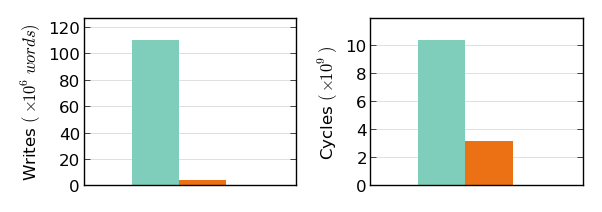
\includegraphics[height=29mm]{./fig/q13_alternate_plan.png} 
}

\subfloat[Overall performance comparison]{ \begin{small}

  %\begin{tabular}{p{3cm}p{2cm}p{2cm}p{2cm}p{2cm}}
  \begin{tabular}{p{3.5cm}c c c c} \toprule                                                                                                
  
  \textbf{Metric} & \textbf{Opt(PCM-O)} & \textbf{Opt(PCM-O) } &
\textbf{Opt(PCM-C)} & \textbf{Opt(PCM-C)}\\ & \textbf{Exec(PCM-O) } &
\textbf{Exec(PCM-C)} & \textbf{Exec(PCM-C)} & \textbf{Exec(PCM-O)}\\ \midrule                                                                                                
  
  \textbf{Mega Word-Writes} &  $233.6$ & $110.6$ & $4.66$ & $12.8$\\
\textbf{Giga Cycles} &  $13.1$ & $10.4$ & $3.2$ & $4.5$\\ \bottomrule
\end{tabular} \end{small} } \caption{Integration with Query Optimization and
Processing Engine} \label{fig:perf_comp} \end{figure}

In light of these modifications, let us revisit Query Q13, for which the
default plan was shown in Figure~\ref{fig:plan_trees}(a). With just the revised
latency costs (i.e. $\lambda$ = 0), the optimizer identified a new execution
plan wherein the merge left-join between the \textit{customer} and
\textit{orders} tables is replaced by a hash left-join.  The relative
performance of these two alternatives with regard to PCM writes and CPU cycles
are shown in Figure~\ref{fig:perf_comp}(a). We observe here that there is a
\emph{huge difference} in both the query response times as well as write
overheads between the plans.  Specifically, the alternative plan reduces the
writes by well over an order of magnitude!  As we gradually increased the
latency slack value, initially there was no change in plans. However, when the
slack was made as large as 5, the hash left-join gave way to a nested-loop
left-join, clearly indicating that the nested-loop join provides write savings
only by incurring a steep increase in latency cost.


To put matters into perspective, Figure~\ref{fig:perf_comp}(b) summarizes the
relative performance benefits obtained as the database layers are gradually
made PCM-conscious (in the figure, the labels Opt and Exec refer to Optimizer
and Executor, respectively, while PCM-O and PCM-C refer to PCM-Oblivious and
PCM-Conscious, respectively). For the sake of completeness, we have also added
results for the case when the Optimizer is PCM-C but the Executor is PCM-O
(last column). The results clearly indicate that future query optimizers for
PCM-based architectures need to incorporate PCM-Consciousness at \emph{both}
the Optimizer and the Executor levels in order to obtain the best query
performance. 

\end{document}


\chapter{Related Work}
\section{Related Work}
\label{relWork}
Over the past decade, there has been considerable PCM-related research
activity on both the architectural front and the various application
domains, including database systems. A review of the literature that is
closely related to our work is presented here.

On the architectural side, buffer management strategies to reduce PCM
latency and energy consumption have been discussed in \cite{lee}. Wear
levelling algorithms are proposed in \cite{wear} that rotate the lines
within a circular buffer each time a certain write threshold is reached. A
randomized algorithm was introduced to handle the case when the writes
are spatially concentrated to enable wear levelling across the entire
PCM. Techniques to reduce writes by writing back only modified data to PCM
upon eviction from LLC/DRAM are presented in~\cite{qureshi,write,lee,zhou}. 
In Flip-N-Write scheme \cite{flipnwrite}, a modified data word
or its complement is stored depending on whose Hamming distance to the
original word is less. As a result, it restricts the maximum bit writes
per word to $B/2$, where \textit{B} is the number of bits in a word.

Turning our attention to the database front, for
the \modelPcmRam{} memory model, write reduction techniques for index
construction and for hash join are proposed in \cite{chen}. They recommend
keeping the keys unsorted at the leaf nodes of the index. While this
scheme saves on writes, the query response times are adversely impacted
due to the increased search times.  Similarly, for partitioning during
hash join, a pointer based approach is proposed to avoid full tuple
writes. Since we assume database to be PCM-resident, this partitioning
step is obviated in our algorithms. A predictive $B^+$ tree is proposed in \cite{hupredictive} 
which pre-allocates node space based on current key distribution which 
helps in reducing write cost due to node splits.

For the \modelExplicit{} memory model, two classes of sort and
join algorithms are presented in \cite{viglas}.  The first class
divides the input into ``write-incurring'' and ``write-limited''
segments. The write-incurring part is completed in a single pass
whereas the write-limited part is executed in multiple iterations.
In the second class of algorithms, the materialization of intermediate
results is deferred until the read cost (in terms of time) exceeds
the write cost.  Our work fundamentally differs from these approaches
since in our \model{} model, there is no explicit control over DRAM.
This means that we cannot selectively decide what to keep in DRAM at any
point of time. It also implies that we may ultimately end up obtaining
much less DRAM space than originally anticipated, due to other programs
running in parallel on the system. As shown in Section \ref{sec:exp},
our algorithms have been designed such that even with restricted memory
availability, they perform better than conventional algorithms in terms
of writes. 

At a more specific level, the sorting algorithms proposed in \cite{viglas}
employ a heap that may be constantly updated during each pass. If the
available DRAM happens to be less than the heap size, it is likely
that the updated entries will be repeatedly evicted, causing a large
number of writes. Secondly, the join algorithms proposed in \cite{viglas}
involve partitioning the data for the hash table to fit in DRAM. However,
since the results are written out simultaneously with the join process,
and the result size can be as large as the product of the join relation
cardinalities, it is likely that the hash table will be evicted even
after partitioning.

Sorting algorithms for \modelExplicit{} model are also discussed in
\cite{vamsi}. They split the input range into buckets such that each
bucket can be sorted using DRAM. The bucket boundaries are determined
using hybrid histograms having both depth-bound and width-bound buckets,
the bound being decided depending upon which limit is hit later.
The elements are then shuffled to group elements of the same bucket
together, followed by sorting of each bucket within the DRAM. The
sorting methodology used is quicksort or count-sort based on whether
the bucket is depth-bound or width-bound respectively. A major drawback
with this approach is that there is a high likelihood of an error in
the approximation of the histogram, leading to DRAM overflow in some of
the buckets. This would lead to additional writes since the overflowing
buckets need to be split into adequately small fragments. Besides,
the construction of the histogram itself may incur a number of writes.

Finally, there has also been quite some research on speeding up query
execution in \textit{flash-resident} databases. For instance, incorporation of the
flash read-write asymmetry within the query optimizer is discussed
in \cite{cost_aware}.  Their focus however is restricted to modifying the 
operator cost modelling to suit the flash environment; the optimization process
itself remaining largely unaltered. The use
of a column based layout has been advocated in \cite{graefe} to avoid
fetching of unnecessary attributes during scans. The same layout is also
leveraged for joins by fetching only the columns participating in the
join, deferring full tuple materialization to as late as possible in
the plan tree. External merge sort is recommended for data not fitting
in the DRAM. These techniques, though applicable to a PCM setting,
are orthogonal to our work.


\chapter{Conclusion}
\section{Conclusion}
\label{conclusion}
Designing database query execution algorithms for PCM platforms requires a
change in perspective from the traditional assumptions of symmetric read
and write overheads.  We presented here a variety of minimally modified algorithms
for the workhorse database operators: \emph{sort}, \emph{hash join} and
\emph{group-by}, which were constructed with a view towards simultaneously
reducing both the number of writes and the response time. Through detailed
experimentation on complete TPC-H benchmark queries, we showed that
substantial improvements on these metrics can be obtained as compared
to their contemporary PCM-oblivious counterparts.  Collaterally, the
PCM cell lifetimes are also greatly extended by the new approaches.

Using our write estimators for uniformly distributed data, we presented
a redesigned database optimizer, thereby incorporating PCM-consciousness
in all layers of the database engine. We also presented initial
results showing how this can influence plan choices, and improve the write
performance by a substantial margin.  While our experiments were conducted
on a PCM simulator, the cycle-accurate nature of the simulator makes it
likely that similar performance will be exhibited in the real world as
well. In our future work, we would like to design write estimators that
leverage the metadata statistics to accurately predict writes for skewed
data. Additionally, we wish to design multi-objective
optimization algorithms for query plan selection with provable performance
guarantees.

Overall, the results of this paper augur well for an easy migration of
current database engines to leverage the benefits of tomorrow's PCM-based
computing platforms.




% \input{chap_review}
% \input{chap_skill_elicitation}
% \input{chap_resource_critical}
% \input{chap_team_formation}
% \input{chap_conclusions}

% \backmatter % book mode only
% \appendix
% \include{Appendix1/appendix1}
% \include{Appendix2/appendix2}

\bibliographystyle{plainnat}
%\bibliographystyle{Classes/CUEDbiblio}
%\bibliographystyle{Classes/jmb}
%\bibliographystyle{Classes/jmb} % bibliography style
% \renewcommand{\bibname}{References} % changes default name Bibliography to References
% \bibliography{References/references} % References file
\bibliography{src/sigproc}
\end{document}
